\begin{figure}[t]
\begin{tabular}{cc}
\begin{subfigure}[b]{0.55\textwidth}
\begin{center}
{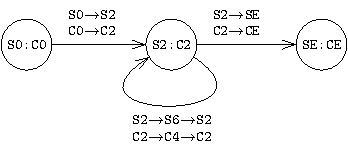
\includegraphics[scale=1]{chapters/figures/figStrlenArrProductCfg.pdf}}
\end{center}
\caption{\label{fig:StrlenArrProductCFG}Product CFG for programs \cref{fig:llStrlenSpecIR,fig:llStrlenCArrIR}}
\end{subfigure}%
&
\begin{subfigure}[b]{0.45\textwidth}
\begin{center}
\begin{scriptsize}
\begin{tabular}{|c|l|}
\hline
\tt PC-Pair & \multicolumn{1}{c|} {\tt Invariants} \\
\hline
\hline
\Tstrut ${\tt (S0:C0)}$ &
${\tt {\circled{P}}\  s_{S}\indEq{}Cstr^{char[]}_{m}(s_{C})}$ \\
\Tstrut \Bstrut \multirow{2}{*}{${\tt (S2:C2)}$} &
${\tt {\scriptsize \circled{I1}}\  s_{S}\indEq{}Cstr^{char[]}_{m}(s_{C})}$ \\ & ${\tt {\scriptsize \circled{I2}}\  len_{S}=i_{C}}$ \\
\Tstrut \Bstrut ${\tt (SE:CE)}$ &
${\tt {\circled{E}}\  ret_{S}=ret_{C}}$ \\
\hline
\end{tabular}
\vspace{5px}
\end{scriptsize}
\end{center}
\caption{\label{fig:StrlenArrInvs}Invariants Table for \cref{fig:StrlenArrProductCFG}}
\end{subfigure}%
\\
\begin{subfigure}[b]{0.55\textwidth}
\begin{center}
{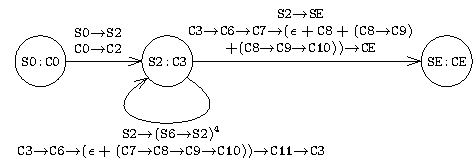
\includegraphics[scale=0.9]{chapters/figures/figStrlenClProductCfg.pdf}}
\end{center}
\caption{\label{fig:StrlenClProductCFG}Product CFG for programs \cref{fig:llStrlenSpecIR,fig:llStrlenCClistIR}}
\end{subfigure}%
&
\begin{subfigure}[b]{0.45\textwidth}
\begin{center}
\begin{scriptsize}
\begin{tabular}{|c|l|}
\hline
\tt PC-Pair & \multicolumn{1}{c|} {\tt Invariants} \\
\hline
\hline
\Tstrut ${\tt (S0:C0)}$ &
${\tt {\circled{P}}\  s_{S}\indEq{}Cstr^{clnode}_{m}(cl_{C}, 0)}$ \\
\Tstrut \Bstrut \multirow{2}{*}{${\tt (S2:C3)}$} &
${\tt {\scriptsize \circled{I1}}\  s_{S}\indEq{}Cstr^{clnode}_{m}(cl_{C}, 0)}$ \\ & ${\tt {\scriptsize \circled{I2}}\  len_{S}=i_{C}}$ \\
\Tstrut \Bstrut ${\tt (SE:CE)}$ &
${\tt {\circled{E}}\  ret_{S}=ret_{C}}$ \\
\hline
\end{tabular}
\end{scriptsize}
\end{center}
\caption{\label{fig:StrlenClInvs}Invariants Table \cref{fig:StrlenClProductCFG}}
\end{subfigure}%
\end{tabular}
\caption{\label{fig:StrlenProductCFGsAndInvs}Product CFGs and Invariants Tables showing bisimulation between Strlen specification in \cref{fig:llStrlenSpecIR} and two C implementations in \cref{fig:llStrlenCArrIR,fig:llStrlenCClistIR}}
\end{figure}